\documentclass{article}
\usepackage{tikz}
\usepackage{pifont}
\usepackage[fontsize=16pt]{fontsize}

\title{Negative Numbers}
\author{Mike McLennan\\
	Applied Scholastics Ferndale\\}
\date{}

\begin{document}

\maketitle
\newpage

\large
\section*{Negative numbers}

Numbers can exist that are less than 0. They are different to the sort of numbers that are used for counting real things.\\

They are called negative numbers and they are written by putting a minus sign to the left of the number. "$-5$" is read as "negative five."\\

Negative numbers can be visualised by extending a number line to the left of 0.\\

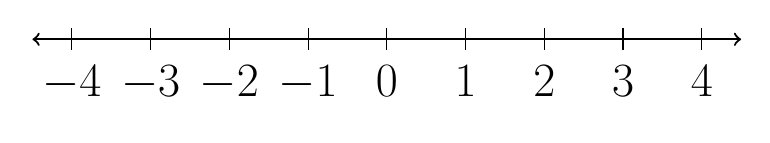
\begin{tikzpicture}
	\draw [<->,thick](-4.5,0) -- (4.5,0);
	\foreach \x in {-4,...,4}
	\draw (\x,4pt) -- +(0,-8pt) node [below] {$\x$};
\end{tikzpicture}

\vspace{16pt}
You can think of them as, instead of having some amount of things, those things are owed as a debt. Say you have 3 of something \ding{46}\ding{46}\ding{46} and someone wants 5 of them \ding{46}\ding{46}\ding{46}\ding{46}\ding{46} there are still 2 more needed. \ding{46}\ding{46}\\

\newpage

Subtraction can be shown by moving to the left on a number line.\\

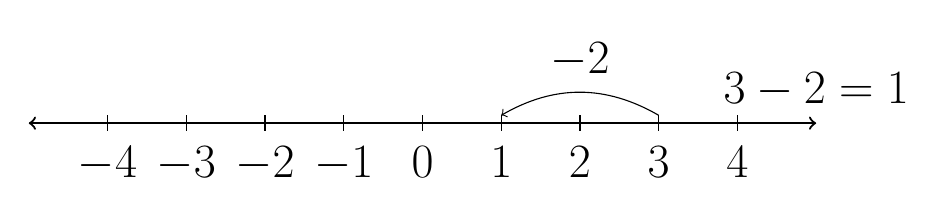
\begin{tikzpicture}
\draw[thick, <->] (-5,0) -- (5,0) node[above] {$3-2=1$};
\foreach \n in {-4,-3,-2,-1,0,1,2,3,4} {\draw (\n,0.1) -- (\n,-0.1) node[below] {$\n$};}
\draw[->, bend right=30] (3,0.1) to node[above] {$-2$} (1,0.1);
\end{tikzpicture}

\vspace{32pt}
You come across negative numbers when subtracting a larger number from a smaller number.\\

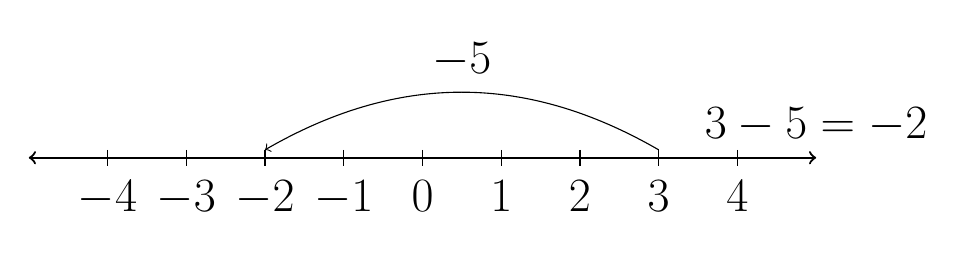
\begin{tikzpicture}
\draw[thick, <->] (-5,0) -- (5,0) node[above] {$3-5=-2$};
\foreach \n in {-4,-3,-2,-1,0,1,2,3,4} {\draw (\n,0.1) -- (\n,-0.1) node[below] {$\n$};}
\draw[->, bend right=30] (3,0.1) to node[above] {$-5$} (-2,0.1);
\end{tikzpicture}

\vspace{32pt}
 With negative numbers the difference between any two numbers can be found, even when the answer is less than 0.\\
 
\newpage

\subsection*{Integers} 
All of the natural numbers plus all of the negative numbers, and zero, are called integers. Integer means ‘untouched,’ meaning that it is a whole amount that hasn't been broken into smaller parts.

\paragraph{Positive Numbers}
Numbers greater than 0 are sometimes called positive numbers, in contrast to the negative numbers. Positive numbers are written with a plus symbol to the left, but of course that is not usually needed. "$+5$" would be read as "positive 5."

\newpage

\section*{Addition}

Adding a negative number to a positive number is the same as subtracting the negative number.

$$5+(-3)=2 \textrm{ is the same as } 5-3=2.$$
$$5+(-8)=-3 \textrm{ is the same as } 5-8=-3.$$

Negative numbers are enclosed in brackets like this when they are written next to other numbers or symbols that could cause confusion.

\section*{Subtraction}

Subtracting a negative number from any other number is the same as adding the negative number.

$$5-(-3)=8 \textrm{ is the same as } 5+3=8.$$
$$(-5)-(-8)=3 \textrm{ is the same as } -5+8=3.$$

\section*{Multiplication}

Multiplying a positive number by a negative number gives a negative product.
$$5\times(-3)=-15.$$

Multiplying a negative number by another negative number gives a positive product.
$$(-5)\times(-3)=-15.$$

\section*{Division}

Dividing a positive number by a negative number, or dividing a negative number by a positive number, both give a negative quotient.
$$15\div(-3)=-5.$$
$$-15\div3=-5.$$

Dividing a negative number by another negative number gives a positive quotient.
$$(-15)\div(-3)=5.$$

\newpage
\
\newpage
\

\begin{center}
\linespread{2}\large

Enquiries

\textbf{Applied Scholastics Ferndale}

Principal: Paula McLennan

mobile phone: 0431 683 306

email address: apsferndale@gmail.com

website: apsferndale.webs.com
\end{center}

\end{document}
